\section{Methods}

\subsection{Feature extraction}
We load the audio signals data using the Python module soundfile. This command
gives us the actual data and the sample rate used. The sample rate in all the
data was 8000Hz.

The features we want are the relative energy ratios of 4 frequency bands:
\(0.0 - 0.5 kHz\), \(0.5 - 1.0 kHz\), \(1.0 - 2.0 kHz\) and \(2.0 - 4.0 kHz\).
We get this by first dividing the audio signal into frames with a length of
30ms, and an overlap of 15ms. With the sampling rate used this means that one
frame has 240 samples.

These frames are then multiplied, or windowed using the Hanning window
function. In figure~\ref{fig:hann50} there's the waveform of the 50th windowed
frame.
\begin{figure}[H]
  \centering
  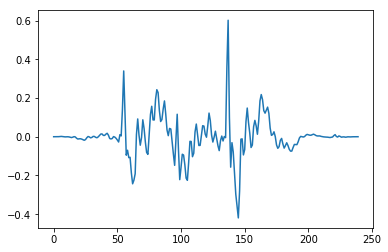
\includegraphics[width=0.8\linewidth]{50-hann-window}
  \caption{50th Hanning-windowed frame}
\label{fig:hann50}
\end{figure}

Then we get the discrete fourier transform of the windowed frames,
with a bin size of 1024. In figure~\ref{fig:amp_spec} there's the amplitude
spectrum of the 50th frame.
\begin{figure}[H]
  \centering
  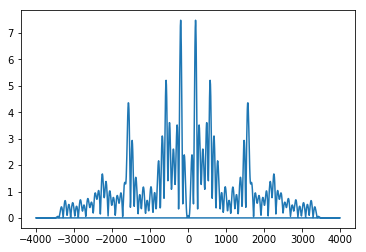
\includegraphics[width=0.8\linewidth]{50-hann-window-fft}
  \caption{Amplitude spectrum of the 50th frame}
\label{fig:amp_spec}
\end{figure}

Out of the frame's DFT we extract the values corresponding to the 4 frequency
bands. For example, the indices of the frequency band \(1-2 kHz\) are 128 to
256. Then we calculate the energy ratio of each band. The energy ratio is
calculated by dividing the energy of a subband by the total energy of that
frame. In figure~\ref{fig:features} there's a visualization of the 50th frames
extracted features.
\begin{figure}[H]
  \centering
  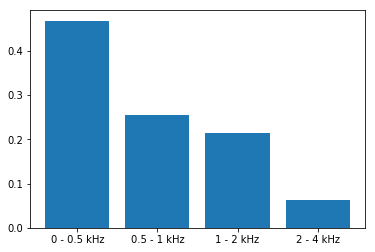
\includegraphics[width=0.8\linewidth]{50-frame-features}
  \caption{Features of the 50th frame}
\label{fig:features}
\end{figure}
Finally, we combine all the frames of a sample by taking the average of all the
frames energy ratios.


\subsection{k-Nearest neighbor classification}

When we have extracted the features, we implement a k-nn classifier as a Python
object. Basically, in the training phase we just copy the data and labels. The
real work is done in the prediction function, where we calculate all the
distances between the sample whose label we're predicting, and all the training
samples. When we have the distances, we take the k-lowest (ie.\ nearest), and
out of those samples we take the most common.

First we classify using only one neighbor. The accuracy was reported by scikit
learn as 69\%. In figure~\ref{fig:conf_mat} we can see the confusion matrix.
The classifier seems to have problems with label number 7, but all in all the
results are pretty good.
\begin{figure}[H]
  \centering
  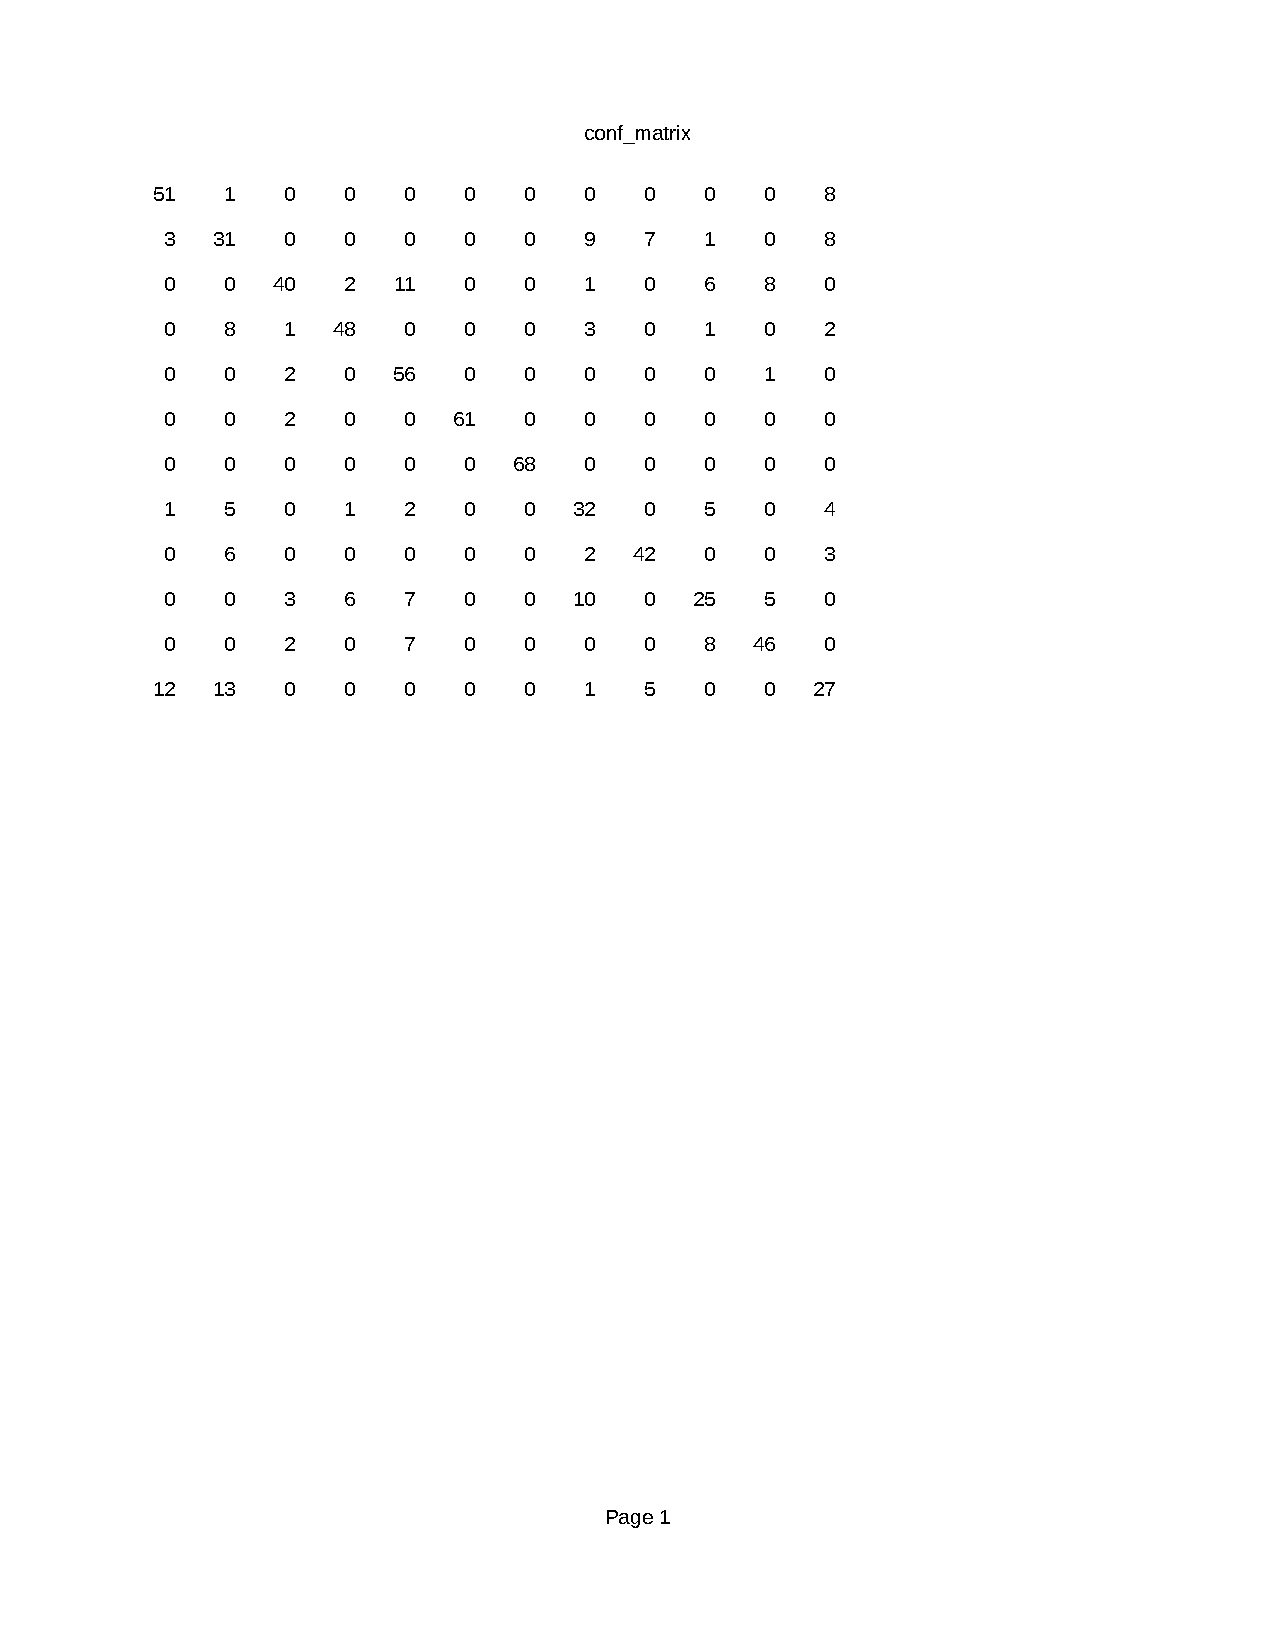
\includegraphics[width=0.8\linewidth]{conf_matrix}
  \caption{Confusion matrix of k=1 classifier}
\label{fig:conf_mat}
\end{figure}


Then we run the classifier with 9 neighbors. This time the accyracy was 70\%.
Figure~\ref{fig:conf_mat_k9} has the confusion matrix of that classifier. No
class sticks out as being very difficult to classify.
\begin{figure}[H]
  \centering
  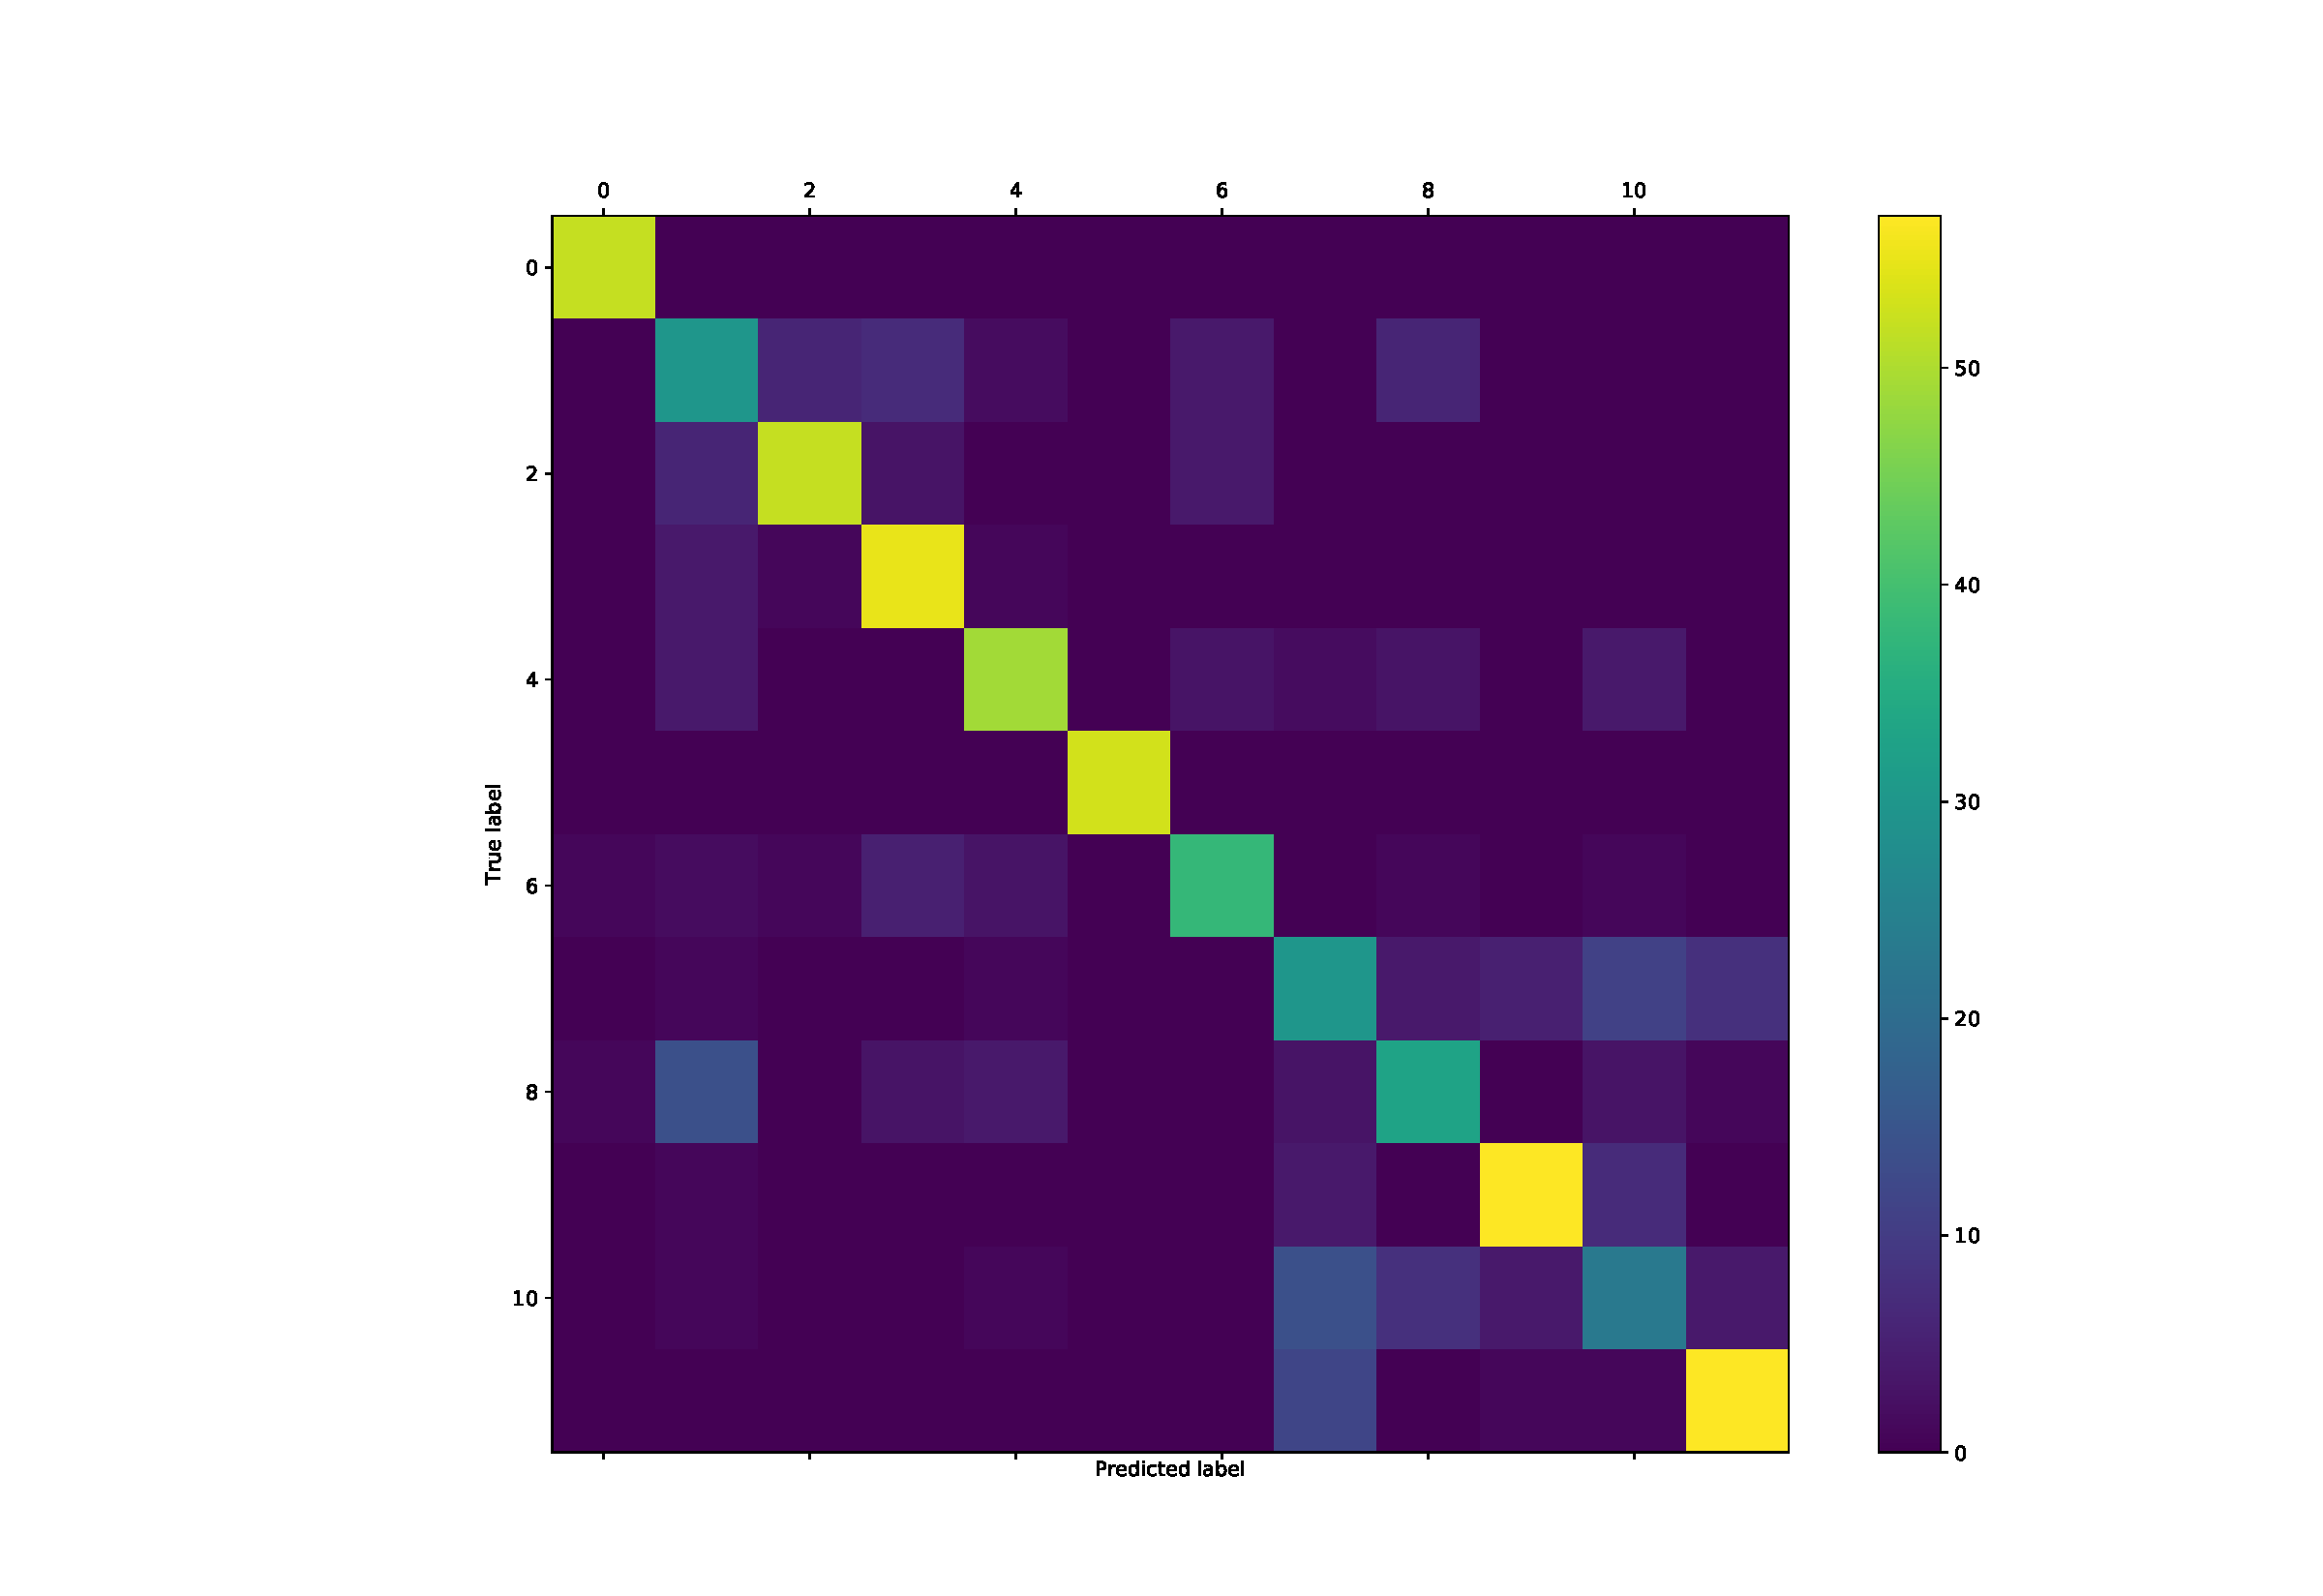
\includegraphics[width=0.8\linewidth]{conf_matrix_k9}
  \caption{Confusion matrix of k=9 classifier}
\label{fig:conf_mat_k9}
\end{figure}









